\documentclass[border=10pt]{standalone}
\usepackage{tikz}
\usetikzlibrary{positioning,arrows.meta,calc,fit}
\begin{document}
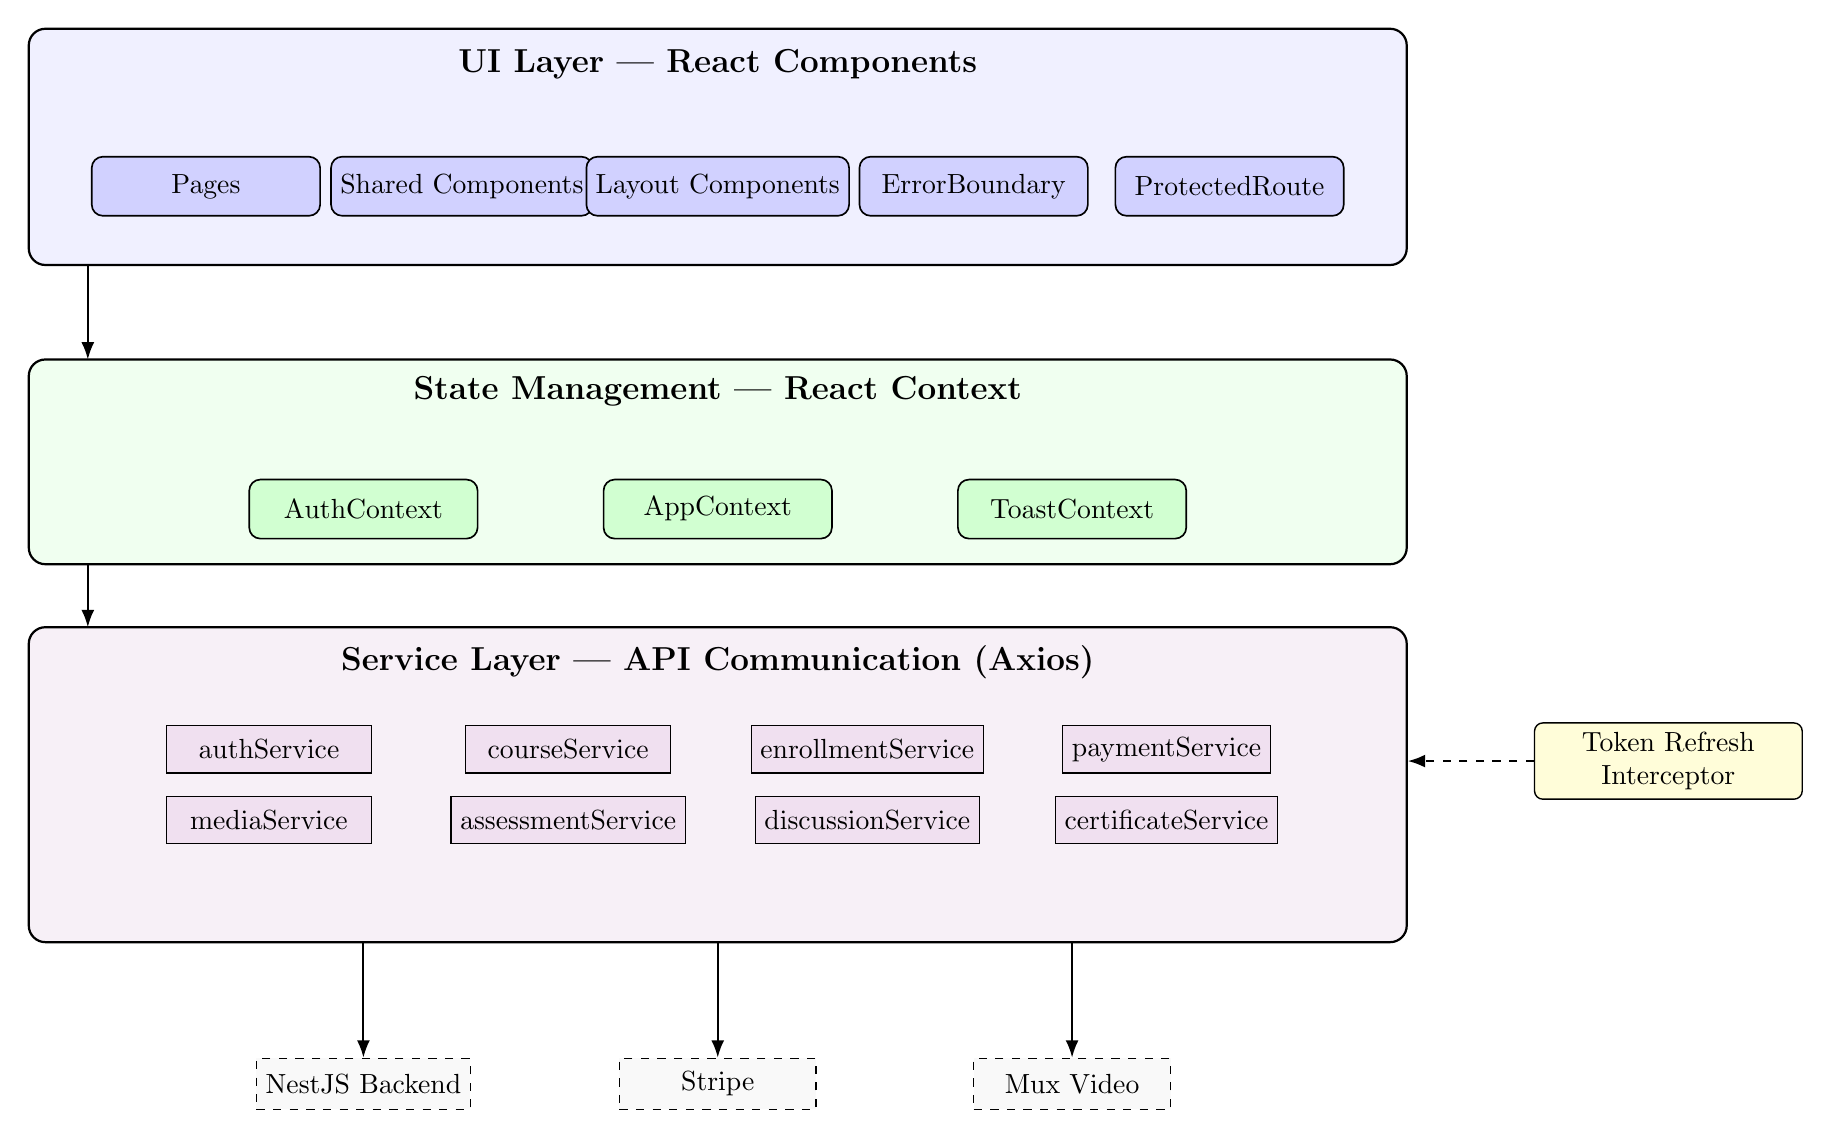
\begin{tikzpicture}[
  font=\normalsize,
  layer/.style={rounded corners=6pt, draw=black, line width=0.8pt, minimum width=17.5cm},
  comp/.style={rounded corners=4pt, draw=black, line width=0.6pt, fill=blue!18, minimum width=2.9cm, minimum height=0.75cm, align=center},
  ctx/.style={rounded corners=4pt, draw=black, line width=0.6pt, fill=green!18, minimum width=2.9cm, minimum height=0.75cm, align=center},
  svc/.style={draw=black, line width=0.5pt, fill=violet!12, minimum width=2.6cm, minimum height=0.6cm, align=center},
  ext/.style={draw=black, line width=0.5pt, dashed, fill=gray!5, minimum width=2.5cm, minimum height=0.65cm, align=center},
  note/.style={rounded corners=3pt, draw=black, line width=0.5pt, fill=yellow!15, align=center, minimum width=3.4cm},
  arr/.style={-{Latex[length=2.2mm]}, line width=0.7pt}
]

%% ---------- Layer 1: UI Components (top edge 13.0, bottom edge 10.0) ----------
\node[layer, minimum height=3.0cm, fill=blue!6] (ui) at (0,11.5) {};
\node[font=\bfseries\large] at (0,12.55) {UI Layer --- React Components};

\node[comp] (pages)   at (-6.5,11.0) {Pages};
\node[comp] (shared)  at (-3.25,11.0) {Shared Components};
\node[comp] (layout)  at (0,11.0)  {Layout Components};
\node[comp] (errb)    at (3.25,11.0)  {ErrorBoundary};
\node[comp] (proute)  at (6.5,11.0)  {ProtectedRoute};

%% ---------- Layer 2: State Management (top edge 8.8, bottom edge 6.2) ----------
\node[layer, minimum height=2.6cm, fill=green!6] (state) at (0,7.5) {};
\node[font=\bfseries\large] at (0,8.4) {State Management --- React Context};

\node[ctx] (authctx)  at (-4.5,6.9) {AuthContext};
\node[ctx] (appctx)   at (0,6.9)    {AppContext};
\node[ctx] (toastctx) at (4.5,6.9)  {ToastContext};

% connector: clear gap 10.0 (ui bottom) to 8.8 (state top), routed off-centre
\draw[arr] (-8.0,10.0) -- (-8.0,8.8);

%% ---------- Layer 3: Service Layer (top edge 5.4, bottom edge 1.4) ----------
\node[layer, minimum height=4.0cm, fill=violet!6] (svclayer) at (0,3.4) {};
\node[font=\bfseries\large] at (0,4.95) {Service Layer --- API Communication (Axios)};

\node[svc] (authsvc)    at (-5.7,3.85) {authService};
\node[svc] (coursesvc)  at (-1.9,3.85) {courseService};
\node[svc] (enrollsvc)  at (1.9,3.85)  {enrollmentService};
\node[svc] (paysvc)     at (5.7,3.85)  {paymentService};

\node[svc] (mediasvc)   at (-5.7,2.95) {mediaService};
\node[svc] (assesssvc)  at (-1.9,2.95) {assessmentService};
\node[svc] (discsvc)    at (1.9,2.95)  {discussionService};
\node[svc] (certsvc)    at (5.7,2.95)  {certificateService};

% connector: clear gap 6.2 (state bottom) to 5.4 (svc top), routed off-centre
\draw[arr] (-8.0,6.2) -- (-8.0,5.4);

%% ---------- External systems ----------
\node[ext] (backend) at (-4.5,-0.4) {NestJS Backend};
\node[ext] (stripe)  at (0,-0.4)    {Stripe};
\node[ext] (mux)     at (4.5,-0.4)  {Mux Video};

\draw[arr] (svclayer.south -| backend) -- (backend.north);
\draw[arr] (svclayer.south -| stripe)  -- (stripe.north);
\draw[arr] (svclayer.south -| mux)     -- (mux.north);

%% ---------- Annotation ----------
\node[note, right=1.6cm of svclayer.east, anchor=west, yshift=0.3cm] (interceptor) {Token Refresh\\Interceptor};
\draw[arr, dashed] (interceptor.west) -- ++(-0.8,0) |- ($(svclayer.east)+(0,0.3)$);

\end{tikzpicture}
\end{document}
